\chapter{Implementation}
This chapter discusses some important aspects of ModelDB S+C's implementation.

\section{System Architecture}
The overall architecture for ModelDB S+C is shown below in Figure 
\ref{fig:system_architecture}.

\begin{figure}
  \centering
  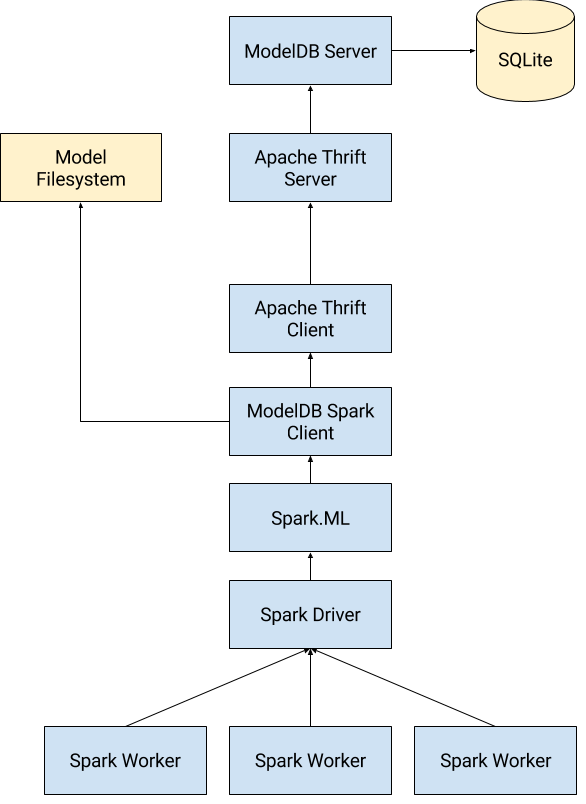
\includegraphics[height=4.0in]{system_architecture}
  \caption{
    The overall architecture of ModelDB S+C. The arrows indicates the flow
    of operations + models data. Notice that the data originates at the Spark workers and
    finds its way into the SQLite database or model filesystem.
  }
  \label{fig:system_architecture}
\end{figure}

In the figure, the operations occur and the models first appear on the Spark worker nodes.
These nodes send their data to the Spark driver node. The driver node runs the Spark.ML
library, which stores objects representing the models and which has functions to trigger
the operations. The ModelDB Spark Client sits on top of the Spark.ML library, and receives the
operations and model data. The Spark Client runs an Apache Thrift client, which it uses to
send data to ModelDB Server. ModelDB Server receives the data, performs the appropriate computations,
and stores it in the SQLite Database. Notice that ModelDB Server does not speak directly to the
model filesystem, which contains the serialized model files. Instead, the Spark Client speaks directly
to the model filesystem. The reasoning for this decision will be discussed later in this chapter.

Recall that ModelDB Server also exposes an API for gleaning information about the model building process.
Spark Client includes convenience functions that the user can call to get this information. In this case,
the arrows would be reversed. When the Spark Client makes a request (via Apache Thrift) to ModelDB Server to run an API 
method, ModelDB Server reads the database, performs the appropriate computations, and responds to the Spark Client. The
Spark Client then extracts the desired information from the response, and returns it to be used in user's driver node
program.

The two key pieces of this diagram are the ModelDB Server and Spark Client. Both
will be discussed below.

\section{Server}
While there is a good deal of code (written in Java) in ModelDB Server, this section will focus only
on interesting pieces of implementation that were not described in the previous chapters.

\subsection{Database}
Currently, ModelDB Server stores its data in a SQLite database. However, it can be
configured to use a number of other SQL databases, like PostgreSQL. This is primarily
achieved by using the JOOQ library. This library asks the user to provide a configuration
file that specifies the database and runs a code generator to create Java classes that
ModelDB Server can use to interact with the database. Changing this configuration file
(and making appropriate changes to the database schema, in order to correct for slight differences
in SQL between languages) can allow ModelDB Server to use a different SQL database than
SQLite. In addition, ModelDB Server is designed to avoid using any esoteric SQLite data types,
functions, or features. Some problems which could be solved by appealing to to a special 
database function are instead solved in ModelDB Server. This places minimal requirements on 
the SQL database that ModelDB Server uses.

\subsection{Model Filesystem}
ModelDB Server allows the user to store their serialized model files in a filesystem. However,
as shown in \ref{fig:system_architecture}, the ModelDB Server does not ever communicate with this
filesystem. Instead, the flow is as follows.

First, the user calls a function in ModelDB Spark Client to indicate that they'd like to save a model and optionally
provides a filename that they would like to use.

Second, the Spark Client indicates to the ModelDB Server that it would like to store the given model under the
given filena,e.

Third, ModelDB Server generates a filepath (incorporating the user's requested filename, if one is provied)
for the model, updates the model's entry in Transformer table 
to reflect this filepath, and sends the filepath to the Spark Client.

Finally, the Spark Client serializes the model and writes the result to the designated filepath.

There are a number of advantages that the above approach has over an approach in which the client
sends the serialized model to the server and the server stores the model in the filesystem. First,
the serialized model file may be large, so storing it directly to the filesystem is cheaper than
first sending it to the server and having the server store the model. Second, some machine learning
libraries (e.g. Spark.ML) store models in a directory structure rather than as a file, and having the
client store the model directly to the given filepath makes this possible. Finally, by pushing the storage
logic to the client, the client could allow the user to provide logic that stores a serialized model
to a completely different filesystem (perhaps their own experimental filesystem). 

\subsection{Configuration}
All the configuration for ModelDB Server (e.g. port to launch server on, prefix for
filepath generation) is defined in a single configuration file, and some sensible defaults
are provided so that ModelDB Server is usuable right out of the box rather than requiring
configuration before use.

\subsection{Stateless, Separated, Logic}
ModelDB Server exposes all its functionality to the client as Thrift endpoints. The client
can make remote procedure calls to this endpoint to store operations, store models, compute 
ancestries, and more. The actual implementation of these Thrift endpoints are extremely short,
most of them being just a single function call. This is done for three reasons. First, it
pushes all of ModelDB Server's logic into other classes, called Data Access Objects (DAOs), 
for which unit tests can be easily written without having to worry about complexities that 
come with using Apache Thrift. Second, it allows ModelDB Server to be used as a library, 
so that other programs could import and use it without having to launch a Thrift server. 
Finally, it makes the server stateless, which can be useful if
future work adds support to scale ModelDB Server to multiple servers.

The ModelDB Server algorithms described in Chapter 4 are each implemented as a single function
or group of functions. They do not persist state between executions and they are expect to have all
their dependencies injected as arguments. The abstractions described in Chapter 3 are implemented as 
SQL tables and also have corresponding Thrift structures to allow them to be sent and received via Thrift
calls.

\section{Spark Client}
The Spark Client is written in Scala, primarily because Spark is written in Java.
Before discussing the implementation details, it is worth seeing a sample usage
of the Spark Client.

\subsection{Sample Usage}
Consider the following sample code, written without ModelDB Spark Client, 
in which a model is trained and evaluated.

\begin{minted}{scala}
val Array(train, test) = data.randomSplit(Array(0.7, 0.3))
val lr = new LogisticRegression()
      .setMaxIter(20)
      .setLabelCol(FeatureVectorizer.indexed(labelCol))
      .setPredictionCol(predictionCol)
      .setFeaturesCol(featuresCol)
val ovr = new OneVsRest()
      .setClassifier(lr)
      .setLabelCol(FeatureVectorizer.indexed(labelCol))
      .setPredictionCol(predictionCol)
      .setFeaturesCol(featuresCol)
val model = ovr.fit(train)
val predictions = model.transform(test)
val eval = new MulticlassClassificationEvaluator()
      .setLabelCol(FeatureVectorizer.indexed(labelCol))
      .setPredictionCol(predictionCol)
      .setMetricName("f1")
val score = eval.evaluate(predictions, model)
\end{minted}

Below, consider the same code WITH ModelDB Spark Client. The changed or
new lines are commented.

\begin{minted}{scala}
// New line.
import edu.mit.csail.db.ml.modeldb.client.ModelDbSyncer._

// New line.
val syncer = ModelDbSyncer.setSyncer(new ModelDbSyncer())

// Use randomSplitSync instead of randomSplit.
val Array(train, test) = data.randomSplitSync(Array(0.7, 0.3))
val lr = new LogisticRegression()
      .setMaxIter(20)
      .setLabelCol(FeatureVectorizer.indexed(labelCol))
      .setPredictionCol(predictionCol)
      .setFeaturesCol(featuresCol)
val ovr = new OneVsRest()
      .setClassifier(lr)
      .setLabelCol(FeatureVectorizer.indexed(labelCol))
      .setPredictionCol(predictionCol)
      .setFeaturesCol(featuresCol)

// Use fitSync instead of fit.
val model = ovr.fitSync(train)

// Use transformSync instead of transform.
val predictions = model.transformSync(test)
val eval = new MulticlassClassificationEvaluator()
      .setLabelCol(FeatureVectorizer.indexed(labelCol))
      .setPredictionCol(predictionCol)
      .setMetricName("f1")

// Use evaluateSync instead of evaluate.
val score = eval.evaluateSync(predictions, model)
\end{minted}

As displayed above, the key changes required to use ModelDB Spark Client are to
import and set up the ModelDB Syncer (the first two lines) and append the suffix
"Sync" to the operations that the user would like to store in ModelDB Server. ModelDB
Spark Client provides "Sync" variants of many Spark.ML methods such as evaluate(),
transform(), fit(), save(), and randomSplit(). Additionally, the ModelDBSyncer
object (called "syncer" in the code sample above) exposes a number of methods for
interacting with ModelDB Server as well (e.g. deserialize a model stored on the
Server, compute ancestry of a DataFrame).

ModelDB Spark Client uses the same types as Spark.ML, so it should interact nicely
with other Spark.ML code and with other libraries that build on Spark.ML. Additionally,
it does not re-implement the functionality of Spark.ML, it only adds functionality. To
understand how this is done, it is worth looking at some aspects of the implementation.

\subsection{Syncable Event}
Recall that a Syncable Event represents an operation that can be stored on ModelDB Server.
The ModelDB Spark Client has a SyncableEvent class that is responsible for converting Spark objects
into their corresponding Thrift structures and then making the appropriate Thrift endpoint call to
store the operation and its primitives on ModelDB Server. Specifically, SyncableEvent is a class
from which many other subclasses derive. These subclasses implement a few methods:

\begin{enumerate}
  \item \textbf{constructor}: The constructor accepts a number of Spark.ML objects (e.g.
  a DataFrame, Estimator, and Transformer, in the case of FitEvent) and sets them as state variables.
  \item \textbf{makeEvent}: This method uses the state variables described above and
  creates a Thrift structure representing the event.
  \item \textbf{sync}: This method calls makeEvent and stores the result on ModelDB Server
  using the appropriate API endpoint. It then passes the result of the API call to the
  associate method.
  \item \textbf{associate}: This method uses the result of the API call to update the
  ModelDBSyncer as appropriate. This includes, for example, updating the ID mappings. The
  ModelDBSyncer is described later in this chapter.
\end{enumerate}

There are SyncableEvent subclasses for all of the Syncable Events that can be stored
on ModelDB Server. These include FitEvent, TransformEvent, MetricEvent, GridSearchCrossValidationEvent,
and more.

\subsection{ModelDBSyncer}
The Spark Client includes a global object called the ModelDBSyncer. This object has a few responsibilities:

\begin{enumerate}
  \item It maintains a buffer of SyncableEvents, which it periodically flushes (by calling sync() on each
  entry of the buffer). The user can configure the syncing strategy (e.g. sync immediately when the buffer contains
  a SyncableEvent, sync only when the ModelDBSyncer is explicitly told to sync).
  \item It exposes convenience functions for interacting with ModelDB Server's API endpoints
  for gleaning information about the model building process (e.g load a deserialized model,
  find the original features that were used to create a model).
  \item It maintains some state about the Spark objects. For example, it stores a mapping between
  Spark objects (e.g. Transformer) to their corresponding IDs in ModelDB Server. This makes it possible to easily get
  the Spark object with a given ID and to get the corresponding ID of a Spark object. Another example, it stores, for
  each DataFrame, the filepath containing the DataFrame's data.
  \item It implements all the traits in the ModelDB Syncer, making it possible to bring all the implicit classes
  into the user's program with just a single import statement.
\end{enumerate}

\subsection{Implicit Classes and Traits}
ModelDB Spark Client aims to augment methods in Spark.ML without having to reimplement or
modify any existing code in Spark.ML. For example, consider the following Spark.ML method:

\begin{minted}{scala}
val model = estimator.fit(dataframe)
\end{minted}

The above method call uses an Estimator to train a model (a Transformer) on a DataFrame.


ModelDB Spark Client includes the following method, which involves the same estimator, dataframe,
and model objects indicated above and each one is the same type as it is in the code sample above.

\begin{minted}{scala}
val model = estimator.fitSync(dataframe)
\end{minted}

This is almost identical in function to Spark.ML's fit method, except that it logs a FitEvent
(or a GridSearchCrossValidationEvent, PipelineEvent if estimator is a CrossValidator or Pipeline,
respectively) to ModelDB Server.

To make the above code possible, ModelDB Spark Client uses a combination of Scala implicit classes
and Scala traits. A Scala trait is similar to an interface in Java or C\#, but it also provide default
implementations for interface methods. A Scala implicit class serves a purpose similar to Java's autoboxing
and unboxing features.

Implementing the fitSync above requires the following:

\begin{enumerate}
\item A Scala trait called SyncableEstimator is defined.
\item Inside SyncableEstimator, a Scala implicit class for Estimator, called EstimatorSync,
is defined. This EstimatorSync implicit class contains an implementation for fitSync(), which calls fit()
on its corresponding Estimator object, creates a FitEvent (a SyncableEvent in Spark Client), and buffers it
onto the global ModelDBSyncer.
\item ModelDBSyncer is marked as implementing the SyncableEstimator trait, so that the EstimatorSync implicit class
is automatically imported into the user's main program. 
\end{enumerate}

Thus, when the user calls fitSync, the following occurs.

\begin{enumerate}
\item Scala looks for an implementation of fitSync() in the Estimator class, and cannot find one.
\item Scala notices there is an implicit class (imported when ModelDBSyncer was imported) 
for Estimator called EstimatorSync that does implement fitSync().
\item Scala creates an EstimatorSync object and passes the Estimator object as a constructor argument.
\item Scala calls the fitSync() method on the EstimatorSync object.
\item Scala returns the result of the fitSync() call, which is the trained model.
\end{enumerate}

This makes it possible augment the Estimator class's fit() function so that it 
buffers a FitEvent in the ModelDBSyncer without having to rewrite or edit existing Spark.ML code.

This technique is used many times in ModelDB Spark Client (e.g. for transformSync(), evaluateSync()).

\subsection{FeatureVectorizer}

ModelDB Spark Client also includes a class called FeatureVectorizer which is a convenience class
for building pre-processing pipelines. The user specifies a DataFrame and indicates the categorical and numerical columns
they'd like to use. Then, FeatureVectorizer builds a PipelineModel that performs common preprocessing steps (e.g. string indexing,
one-hot encoding, standardization of numerical columns) and creates an output DataFrame with a "features" column that can
be used by a machine learning Estimator or Model.

